%% ---------------------------------------------------------------------
\section{Interface reference}
\label{app:reference}

\begin{table}[H]
\centering\small
\caption{ROS~2 topics produced by the ground stack.}
\begin{tabularx}{\textwidth}{p{5.2cm} L}
\toprule
\textbf{Topic} & \textbf{Content} \\
\midrule
\topic{/odom}, TF \code{odom}$\rightarrow$\code{base_link} & Vehicle pose/twist (EKF local position if available, otherwise flow dead-reckoning) \\
\topic{/scan} & \code{LaserScan}, 360 readings at \SI{1}{\degree} \\
\topic{/camera/image_raw} & Camera image \\
\topic{/drone/optical_flow} & Raw flow and ground distance (debug) \\
\topic{/segmentation/detections} & Class, score and box per object \\
\topic{/segmentation/class_mask}, \topic{/instance_mask} & Per-pixel class id + 1 / instance index + 1 \\
\topic{/segmentation/image_annotated} & Annotated image (published only when subscribed) \\
\topic{/cmd_vel} & Nav2 velocity command \\
\topic{/map_3d} & Voxelised 3D point cloud (\code{PointCloud2}, \SI{1}{\hertz}) \\
\topic{/diagnostics}, \topic{/metrics/overlay}, \topic{/metrics/dashboard} & Health summary and RViz overlays \\
\bottomrule
\end{tabularx}
\end{table}

\begin{table}[H]
\centering\small
\caption{Health metrics published under \topic{/metrics/}.}
\begin{tabularx}{\textwidth}{p{6.6cm} L}
\toprule
\textbf{Metric} & \textbf{Meaning} \\
\midrule
\code{{lidar,telemetry,camera}/latency_ms} & One-way Pi$\rightarrow$laptop latency (\cref{eq:latency}), absolute once clocks are synced \\
\code{*/latency_excess_ms} & Latency above the 10\,s-window minimum (clock-independent) \\
\code{*/rate_hz}, \code{lidar/jitter_ms} & Arrival rate and inter-arrival jitter \\
\code{camera/{decode_ms,bandwidth_mbps,dropped_frames}} & Camera cost and load \\
\code{lidar/{nearest_obstacle_m,valid_ratio,tf_fail_ratio}} & LiDAR quality \\
\code{tf/odom_base_age_ms} & Age of the latest pose \\
\code{costmap/local/scan_agreement} & \Cref{eq:agreement}; $\approx$1 when costmap matches LiDAR \\
\code{costmap/{local,global}/{rate_hz,lethal_cells}} & Costmap update rate and obstacle count \\
\code{odom/{speed_mps,distance_from_start_m,path_length_m}} & Motion and drift indicators \\
\code{flow/{quality,ground_distance_m}} & Optical-flow sensor state \\
\code{nav/{cmd_vel_rate_hz,cmd_speed_mps,plan_length_m}} & Planner activity \\
\code{segmentation/{inference_ms,yolo_ms,sam_ms,sam_refined}} & Perception cost and output \\
\bottomrule
\end{tabularx}
\end{table}

\begin{table}[H]
\centering\small
\caption{Options of \code{start_streams.py} (companion).}
\begin{tabularx}{\textwidth}{p{4.6cm} p{3.2cm} L}
\toprule
\textbf{Option} & \textbf{Default} & \textbf{Effect} \\
\midrule
\emph{laptop IP} (positional) & SSH client / gateway & Destination of all streams \\
\code{--nav-cmds} & off & Enable Nav2 velocity forwarding (armed + GUIDED only) \\
\code{--no-telemetry/--no-lidar/--no-camera} & -- & Omit a stream \\
\code{--pixhawk-port} & \code{/dev/pixhawk} & Autopilot device \\
\code{--lidar-port}, \code{--lidar-baud} & \code{/dev/ttyUSB0}, 115200 & LiDAR serial \\
\code{--camera-device}, \code{--camera-size} & \code{/dev/camera}, 640x480 & Camera and resolution \\
\code{--fps}, \code{--quality} & 20, 70 & Camera rate, JPEG quality \\
\code{--camera-passthrough} & off & Forward camera MJPEG without re-encoding \\
\code{--rate} & 30 & Max telemetry rate (Hz) \\
\code{--keep-powersave}, \code{--no-time-sync} & off & Skip Wi-Fi power-save change / clock sync \\
\bottomrule
\end{tabularx}
\end{table}

\begin{table}[H]
\centering\small
\caption{Arguments of \code{navigation_real.launch.py} (ground).}
\begin{tabularx}{\textwidth}{p{3.4cm} p{3.6cm} L}
\toprule
\textbf{Argument} & \textbf{Default} & \textbf{Effect} \\
\midrule
\code{pi_ip} & \code{$GPS_DENIED_PI_IP} & Companion address for commands \\
\code{camera}, \code{segmentation} & true, true & Camera receiver; YOLO+SAM node \\
\code{seg_model}, \code{seg_sam_model} & \code{yolov8n-seg.pt}, \code{sam2.1_t.pt} & Weights (\code{none} disables SAM) \\
\code{seg_sam_imgsz} & 768 & SAM input size (1024 = sharpest) \\
\code{rviz}, \code{metrics}, \code{map3d} & true & Visualisation, health monitor, 3D mapper \\
\code{params_file} & \code{config/nav2_real.yaml} & Nav2 parameters \\
\code{use_sim_time} & false & Simulation clock \\
\bottomrule
\end{tabularx}
\end{table}

\section{Reproducing the validation figures}
\label{app:repro}

\begin{lstlisting}[language=bash]
cd gps-denied-vtol
# segmentation timing (needs CUDA GPU, ultralytics, weights in ros2_ws/)
python3 report/scripts/bench_segmentation.py --iters 100
# bench-log figures, ZUPT and dead-reckoning analysis
python3 report/scripts/make_figures.py      # writes report/figures/*.pdf, data/bench_stats.txt
python3 report/scripts/make_extra_figures.py # latency, delivery, drift and KPI summary figures
# segmentation unit tests
cd ros2_ws/src/quadcopter_perception
PYTEST_DISABLE_PLUGIN_AUTOLOAD=1 python3 -m pytest test/test_hybrid_segmenter.py
# trade-study charts
python3 scripts/analysis.py
\end{lstlisting}

\section{Additional trade-study views}
\label{app:trade}

Cost and robustness views of the screening data in \cref{tab:solutions}.

\begin{figure}[H]
\centering
\begin{subfigure}[t]{0.49\textwidth}
  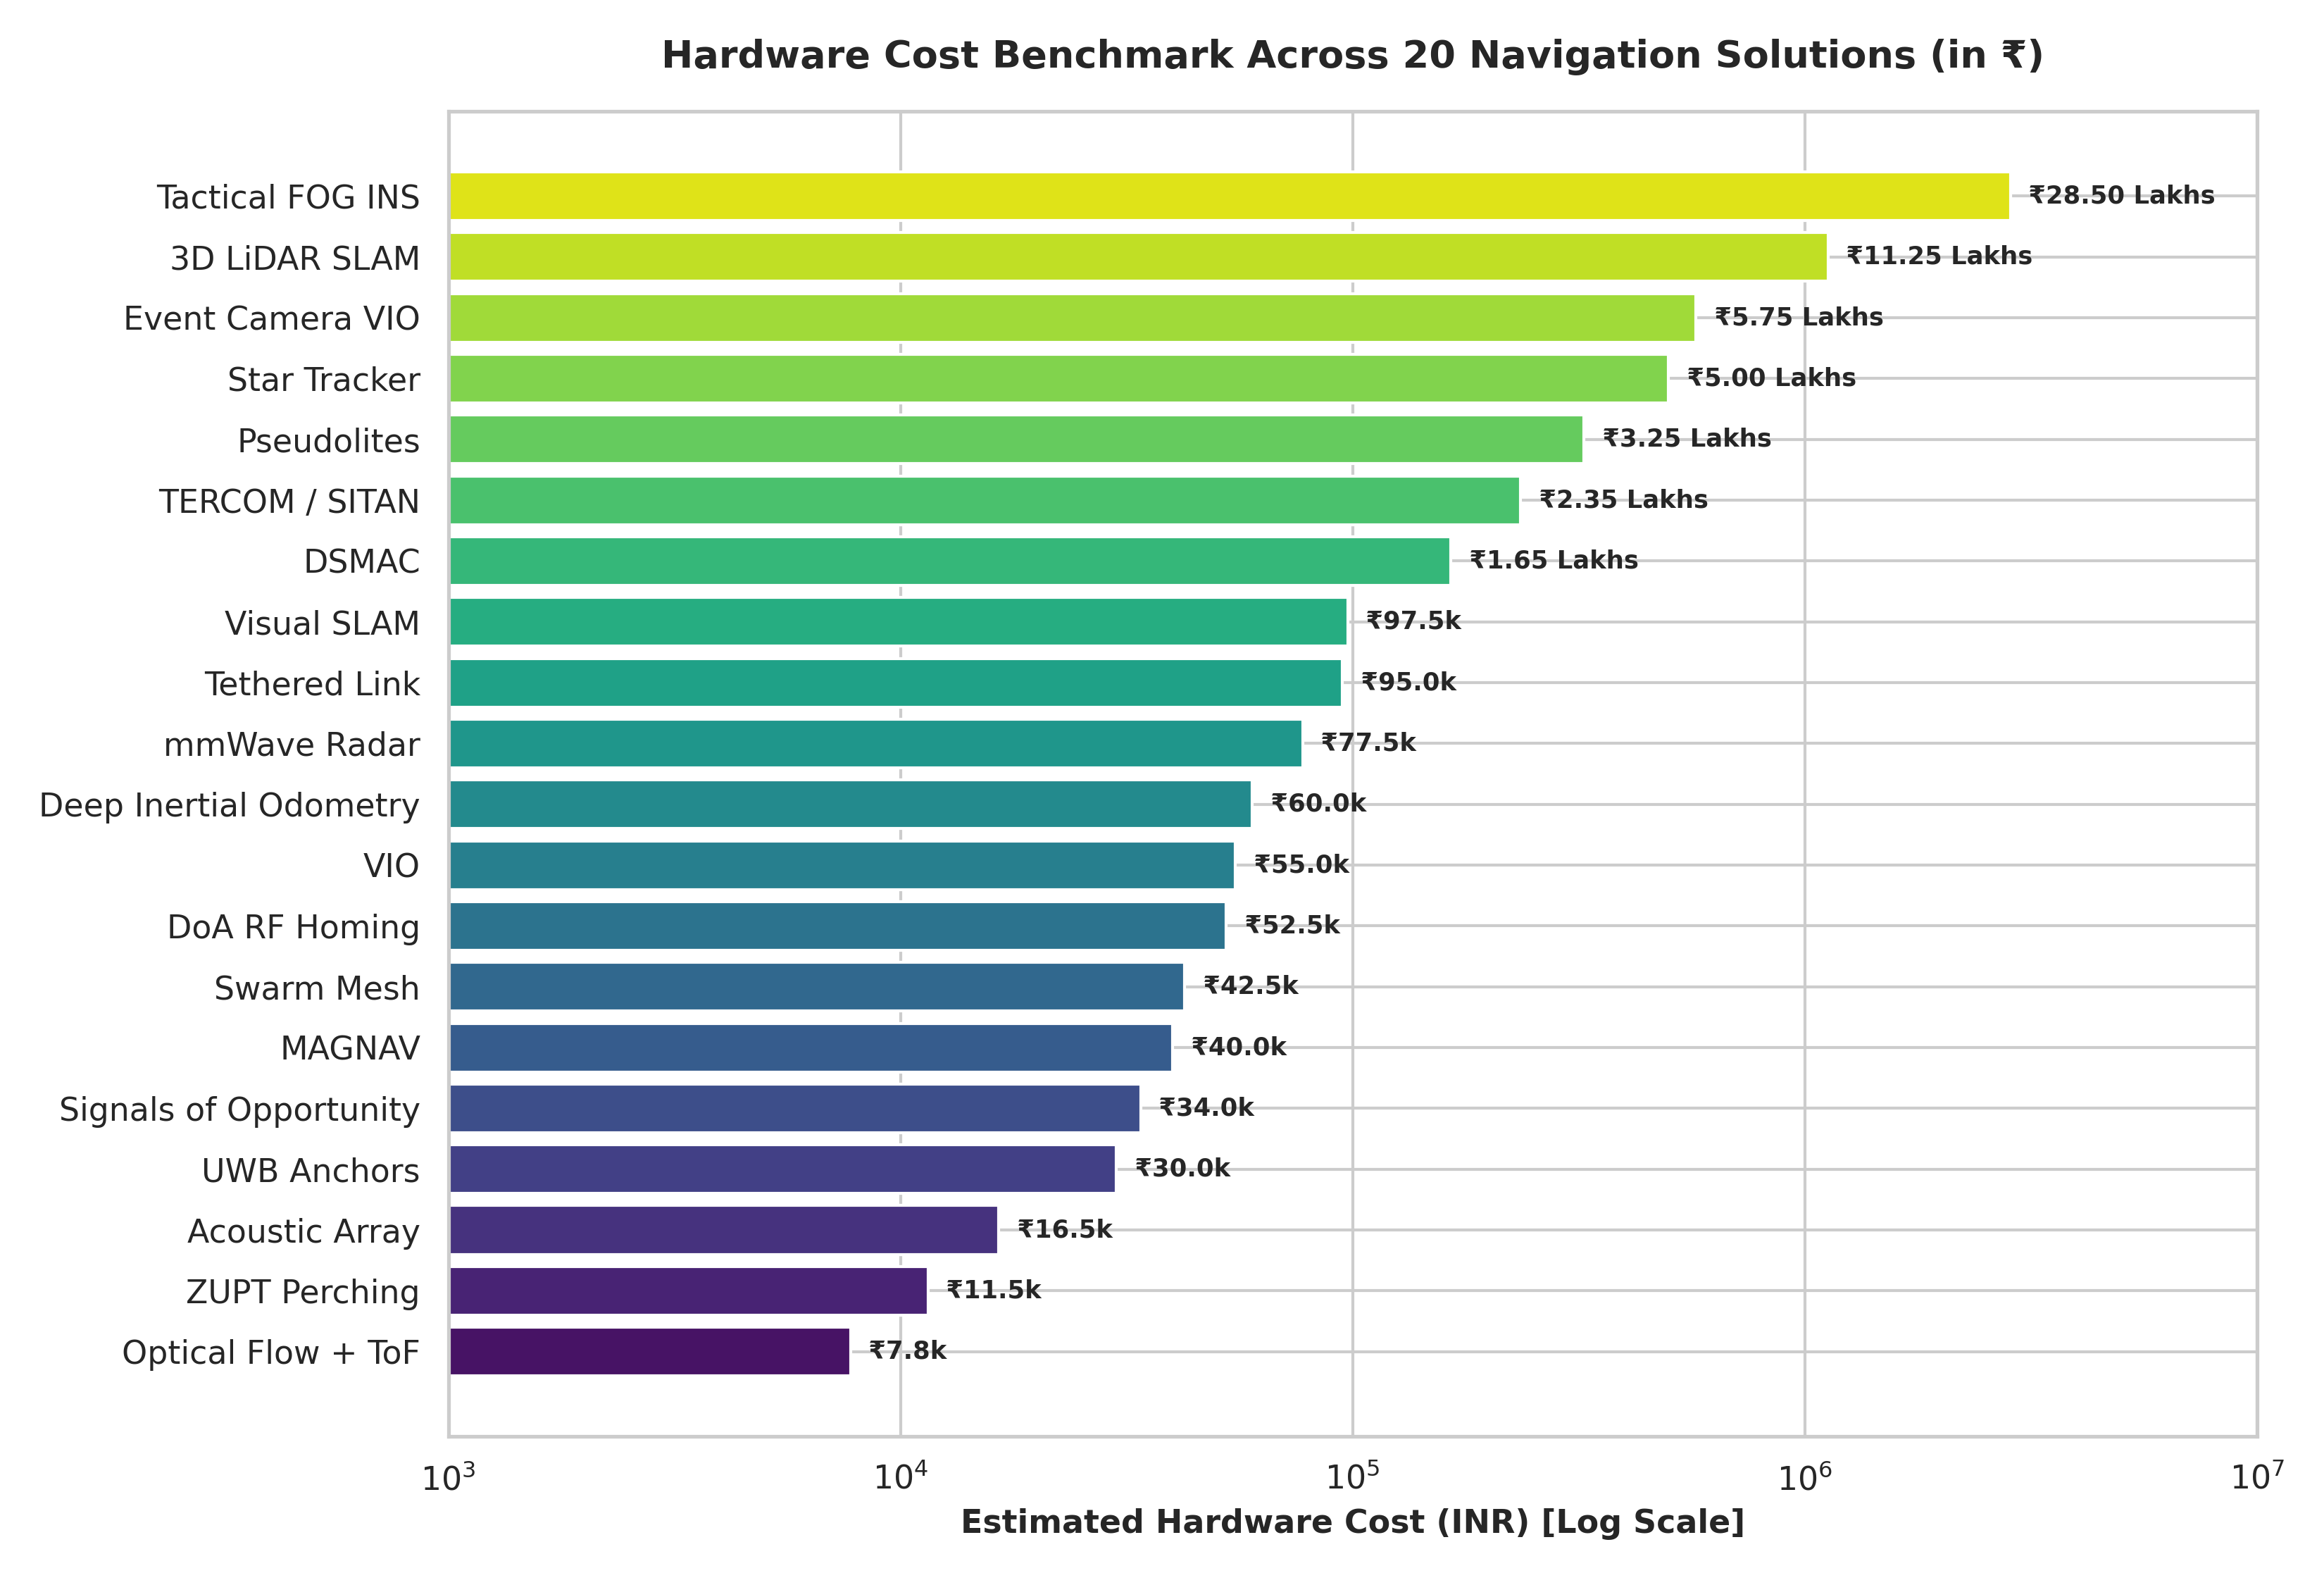
\includegraphics[width=\linewidth]{3_cost_benchmark_inr.png}
  \caption{Hardware cost per solution (INR, log scale).}
\end{subfigure}\hfill
\begin{subfigure}[t]{0.49\textwidth}
  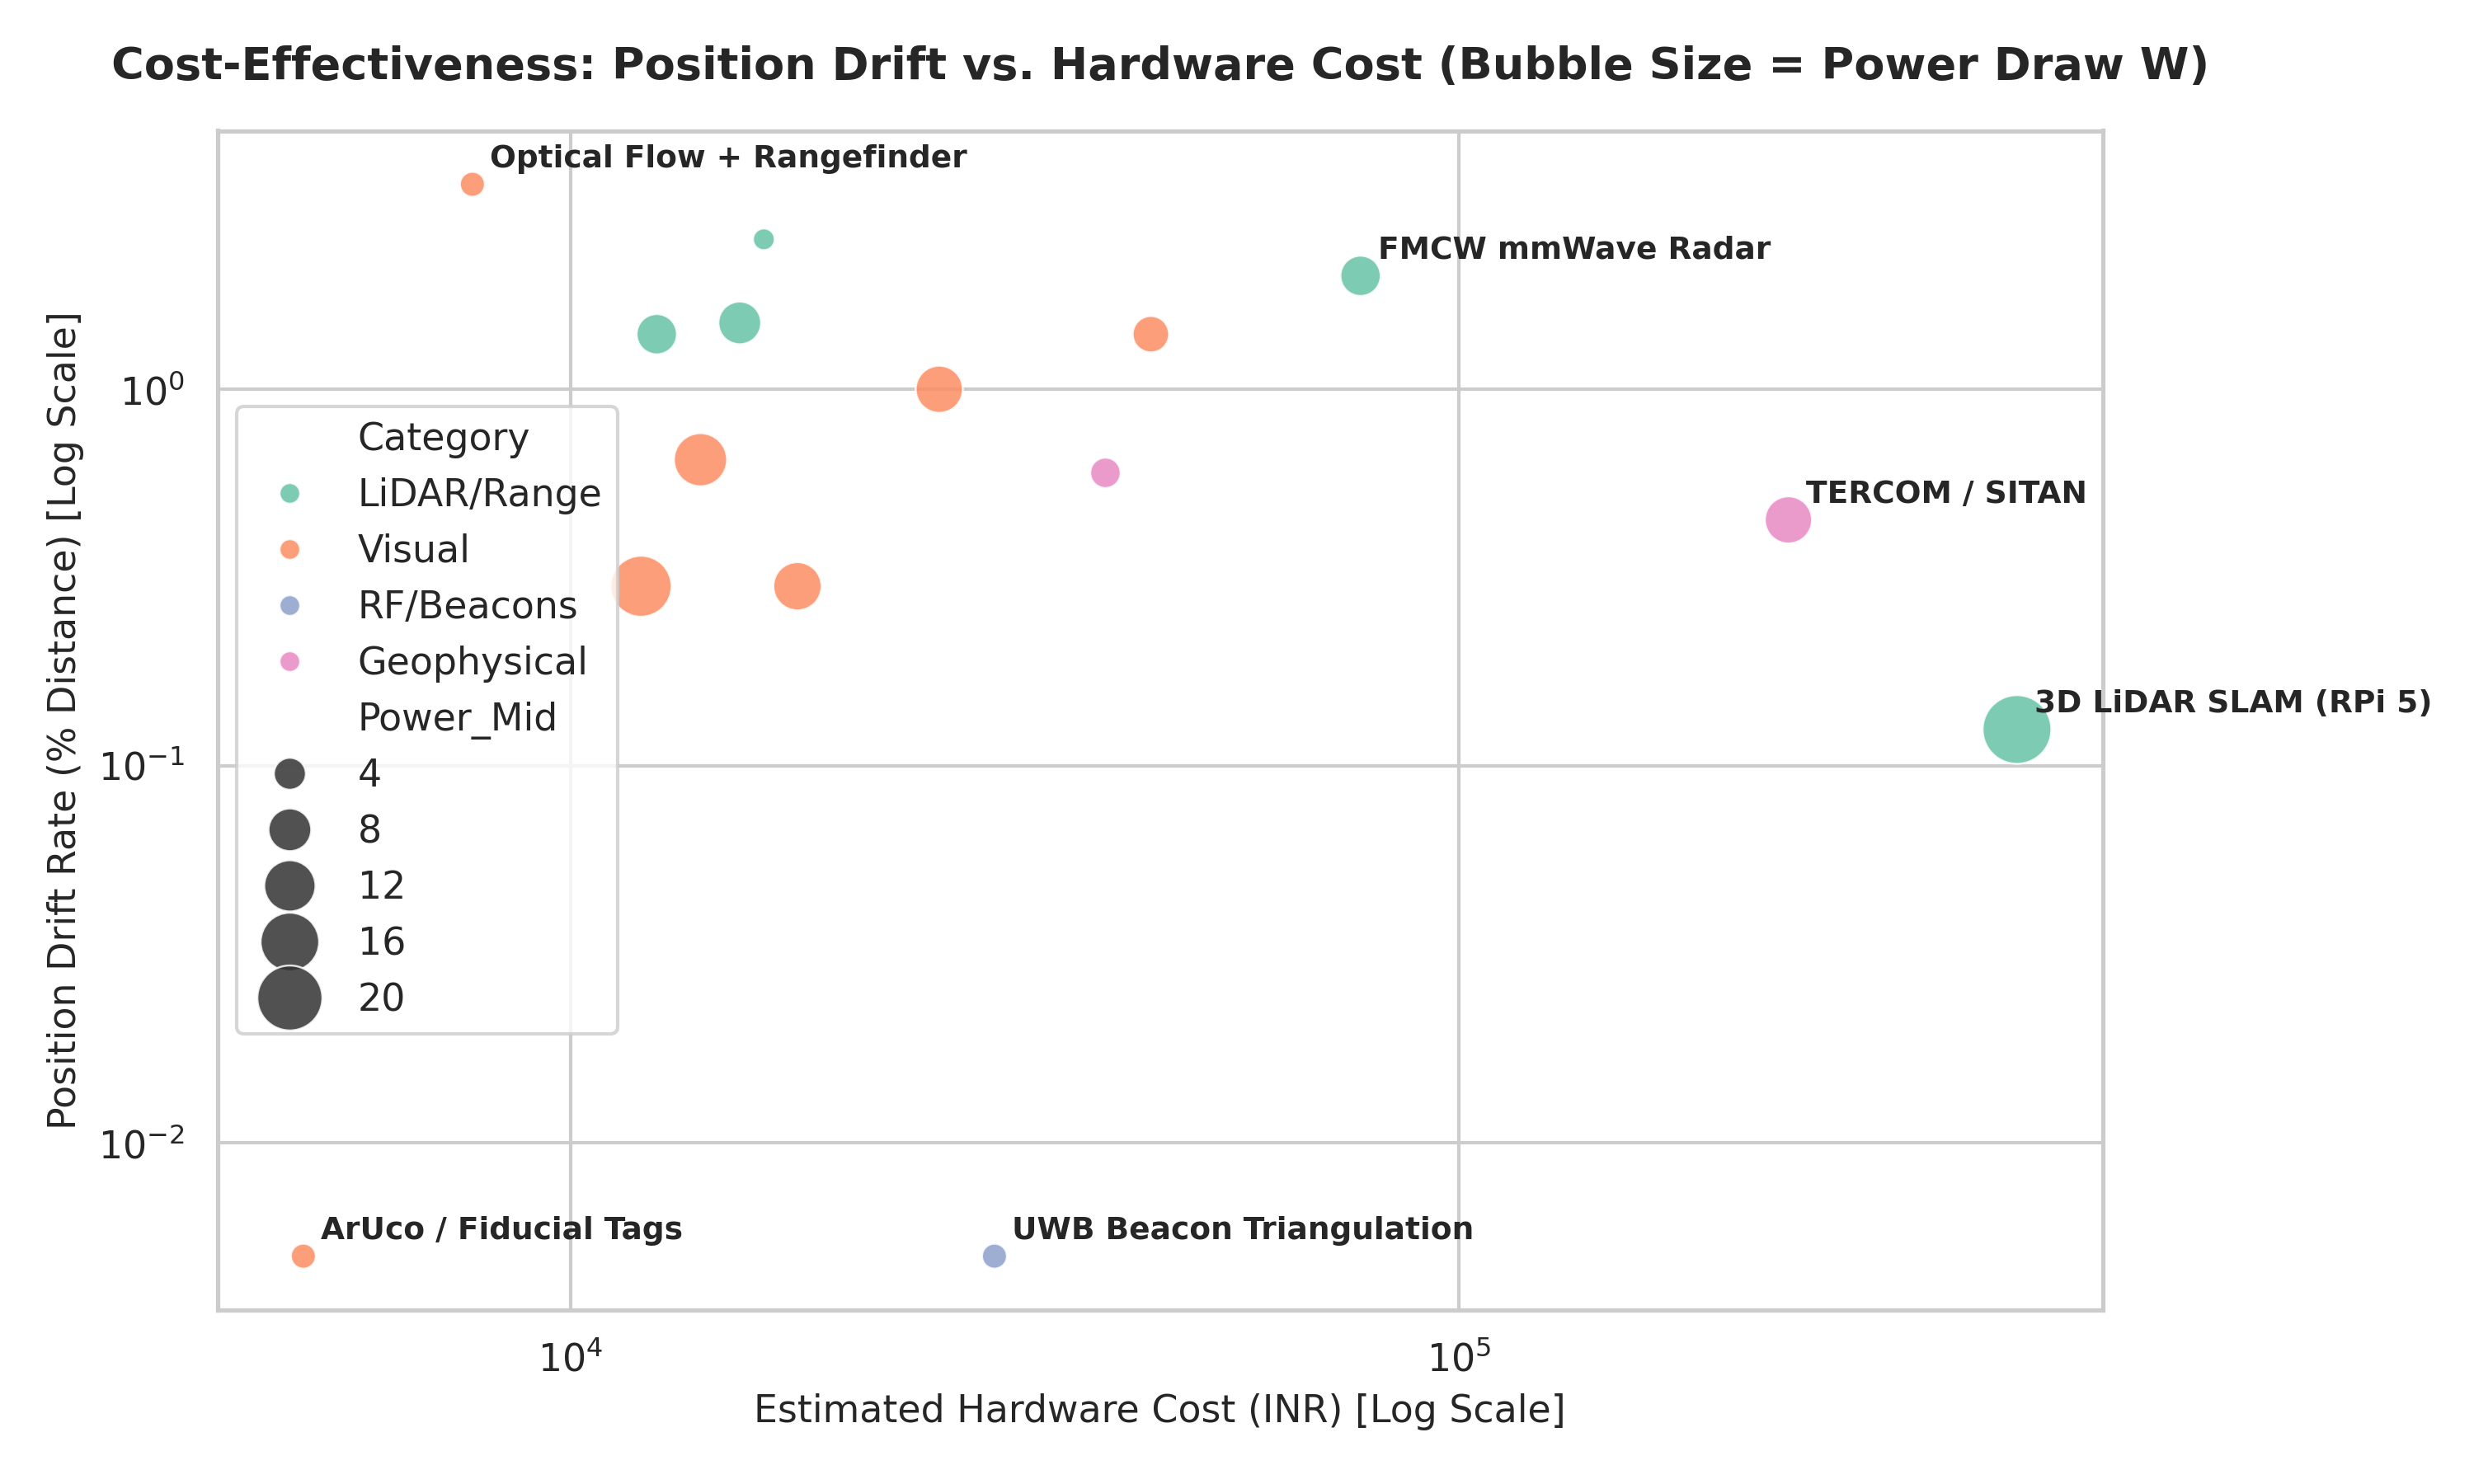
\includegraphics[width=\linewidth]{5_cost_effectiveness.png}
  \caption{Drift against cost (bubble size = power).}
\end{subfigure}

\vspace{2mm}
\begin{subfigure}[t]{0.49\textwidth}
  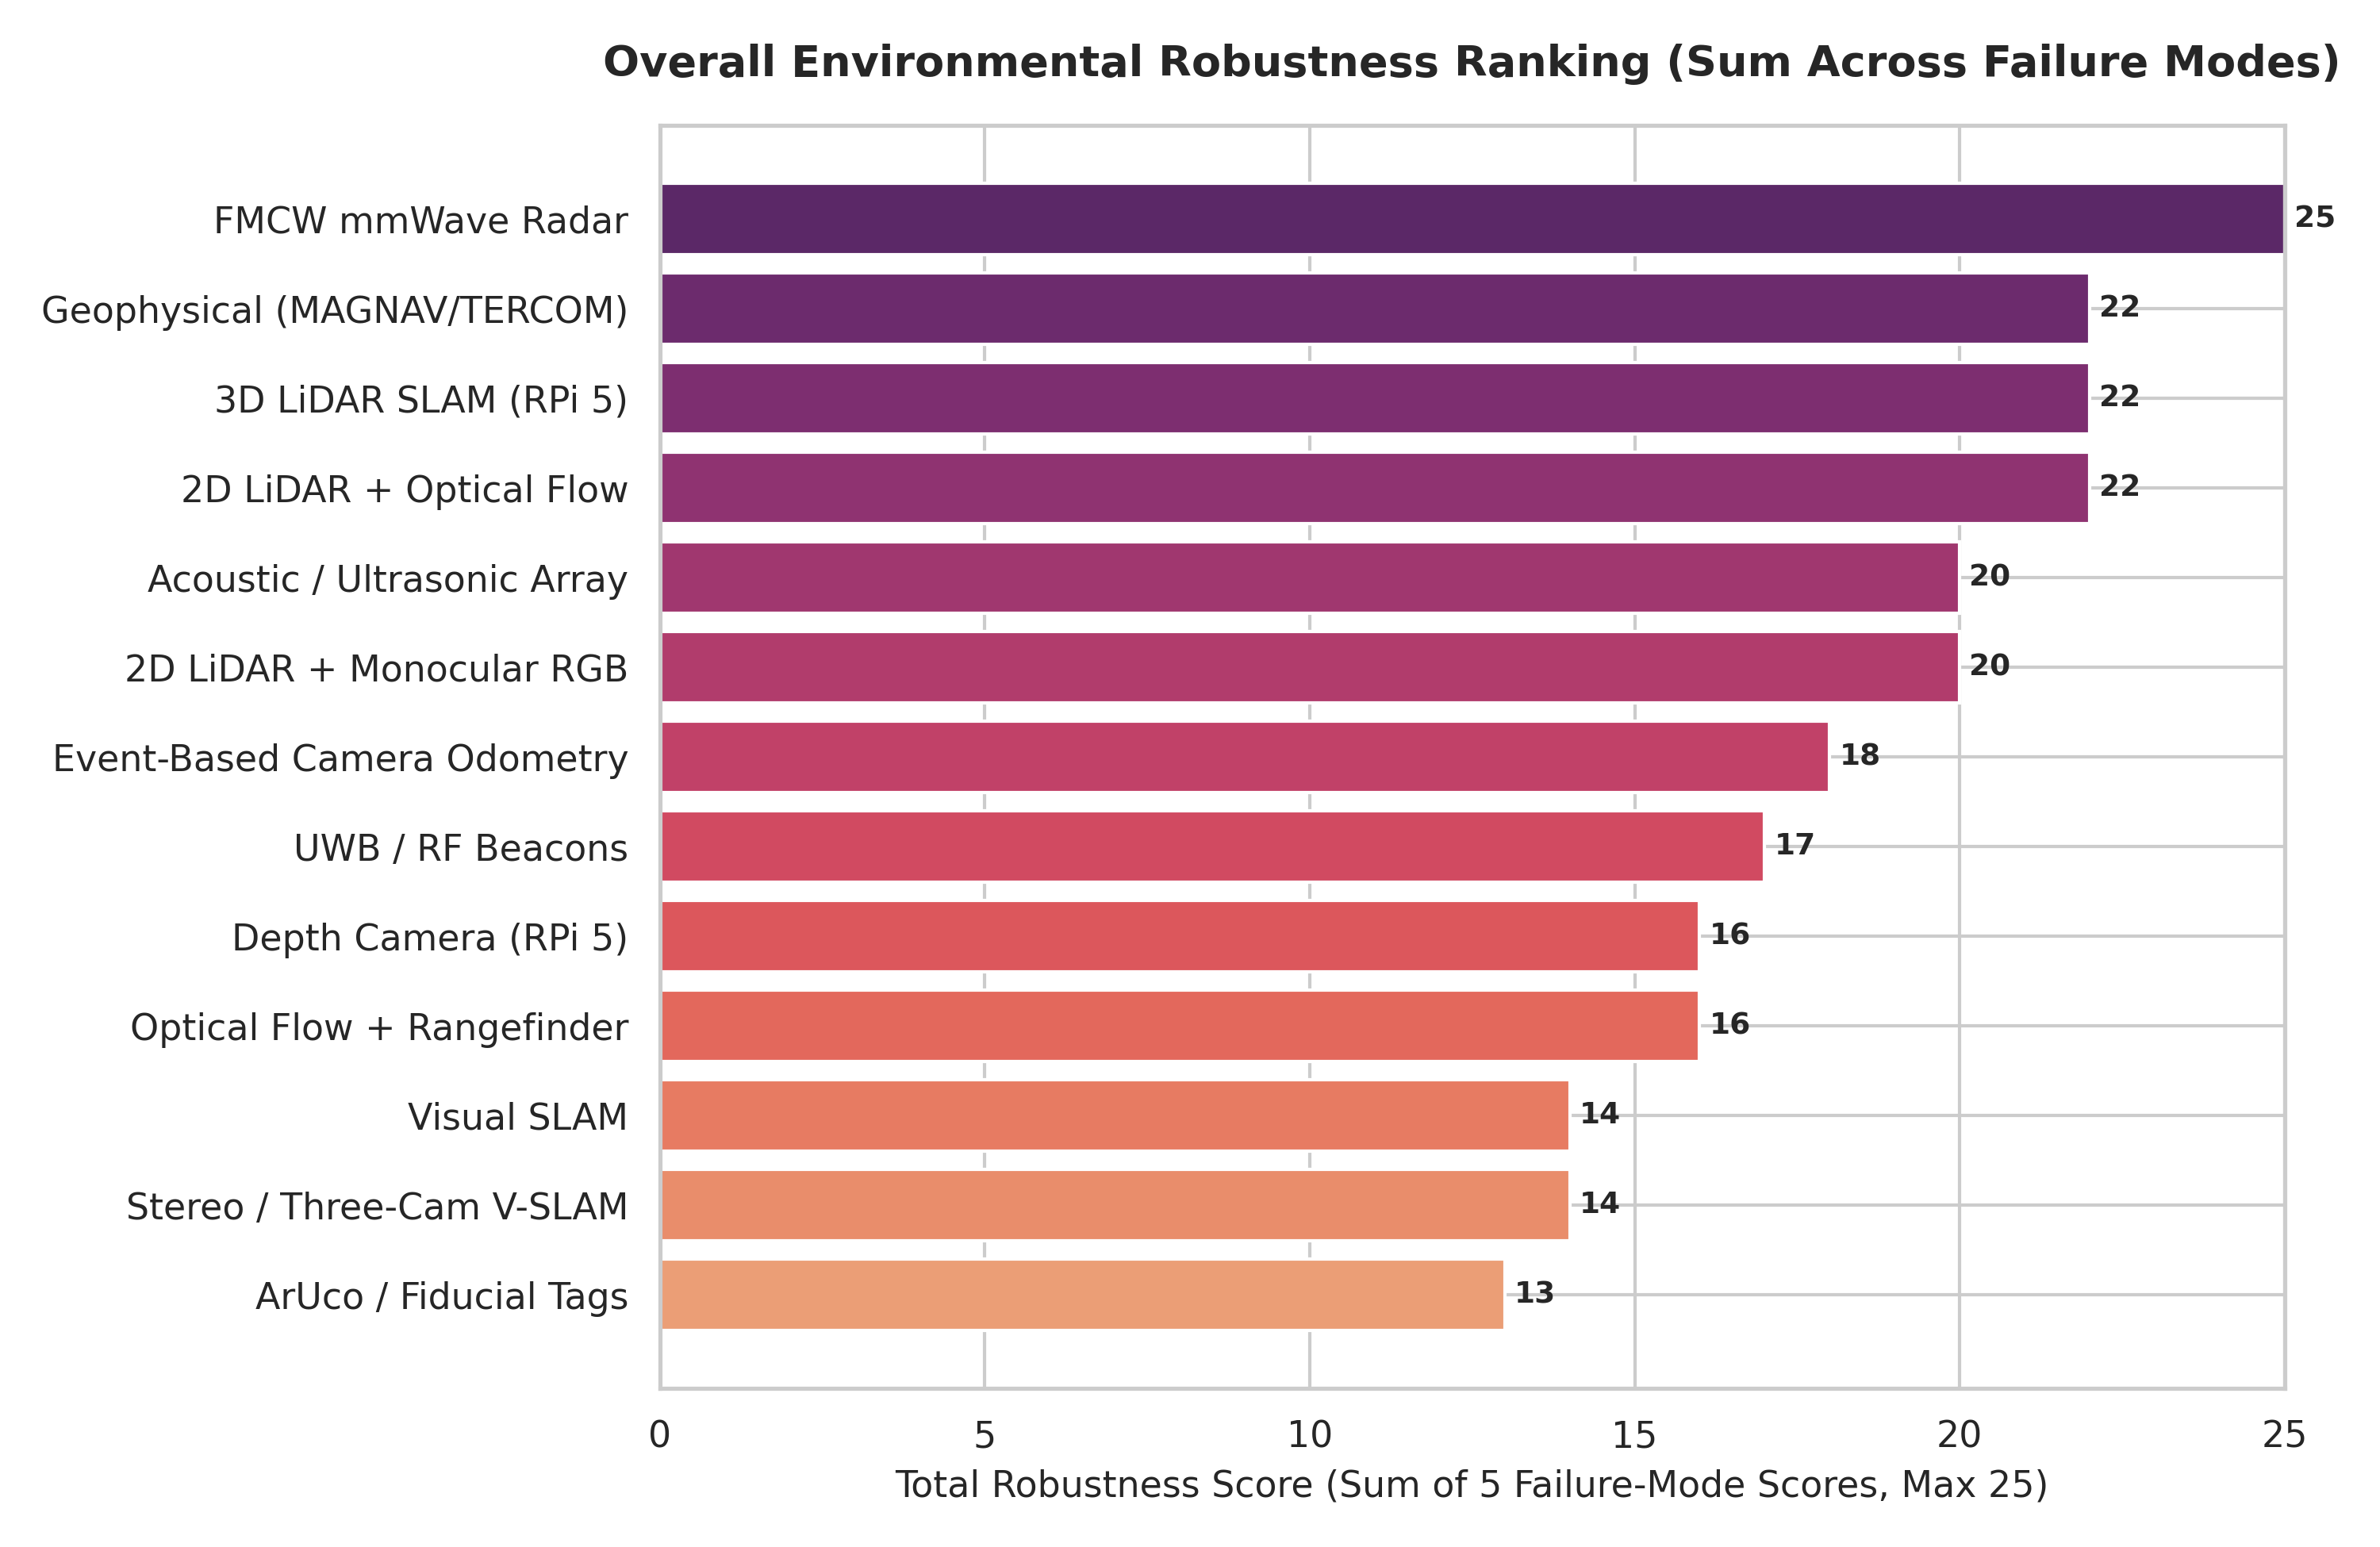
\includegraphics[width=\linewidth]{7_robustness_total.png}
  \caption{Total robustness score (sum of five failure modes).}
\end{subfigure}\hfill
\begin{subfigure}[t]{0.49\textwidth}
  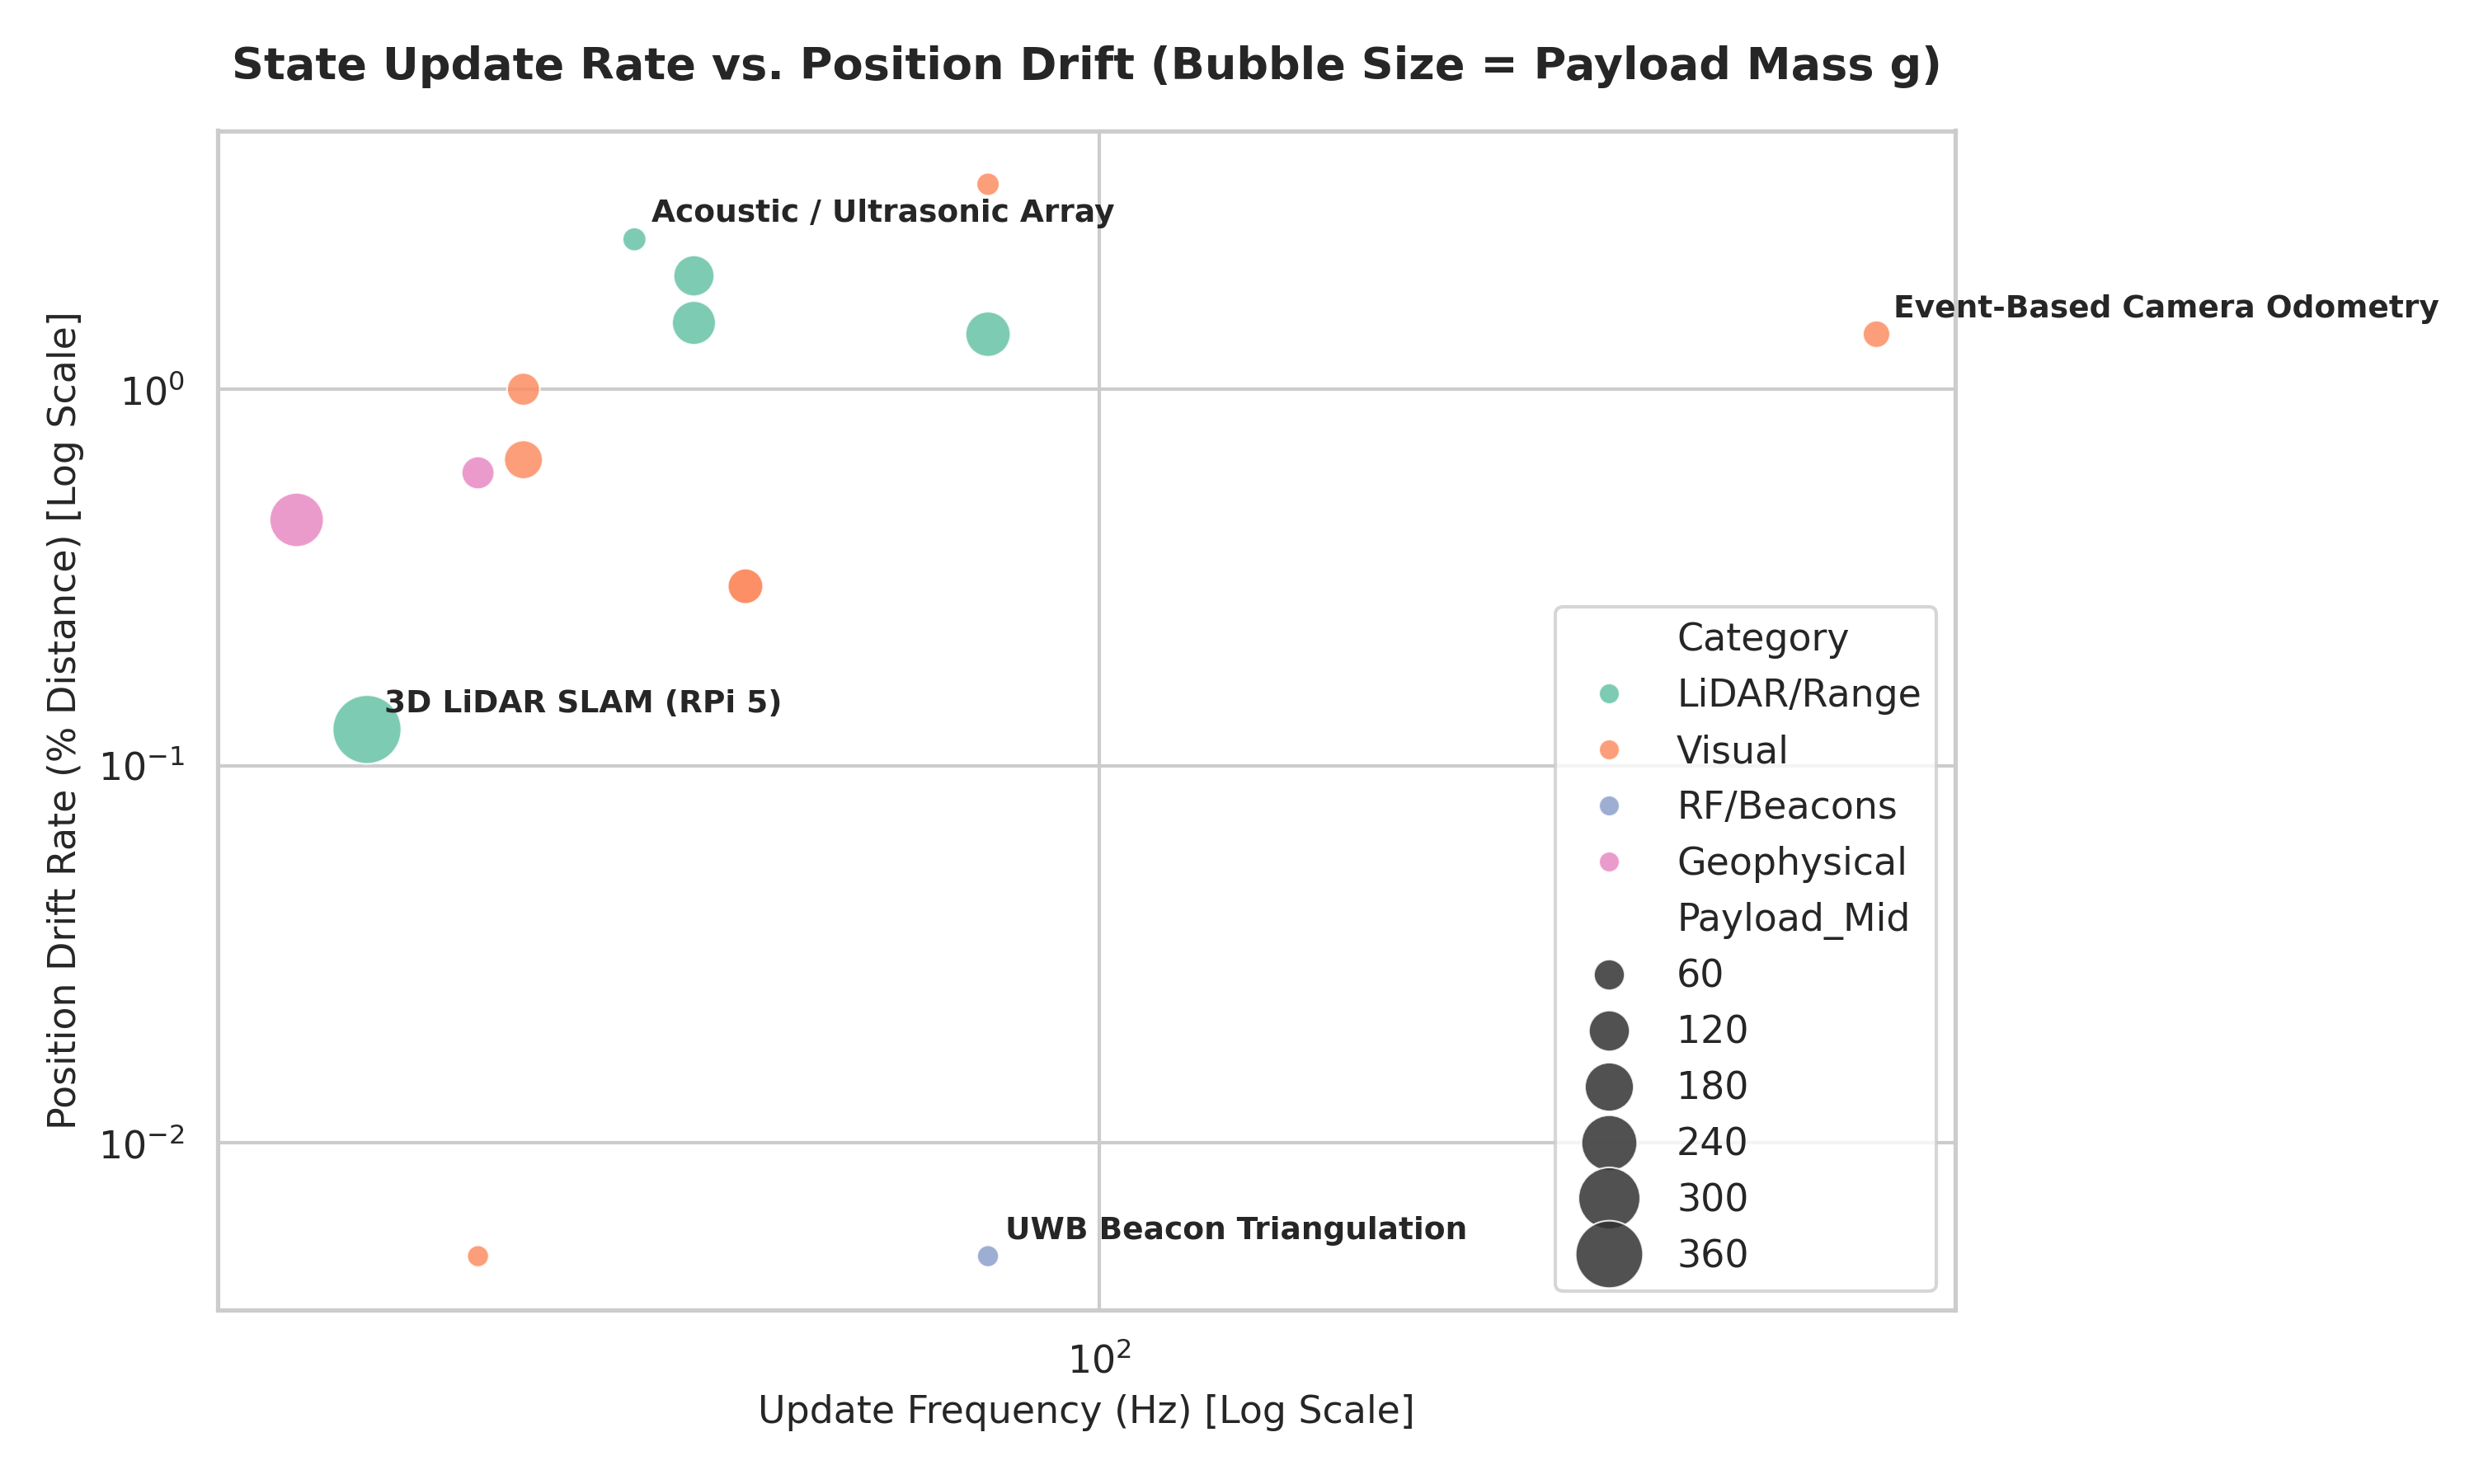
\includegraphics[width=\linewidth]{10_update_rate_vs_drift.png}
  \caption{Update rate against drift (bubble size = mass).}
\end{subfigure}
\caption{Further views of the same trade-study dataset (\cref{tab:solutions}), from
\code{scripts/analysis.py}. The values are screening estimates, not measurements.
Axes with drift or cost use log scales.}
\label{fig:trade2}
\end{figure}
